\section{Modélisation}

\subsection{Clustering}

\subsubsection{Workflow}

Le pipeline de travail permet de clusteriser le jeu de données suivant
différents axes, que l'on peut sélectionner facilement en filtrant les
colonnes d'attributs en début de chaîne. Les attributs retenus sont
normalisés sur l'intervalle $[ 0 ; 1 ]$. On s'assure qu'aucune valeur
manquante ne reste dans un des attributs en enlevant la ligne concernée
(les attributs étudiés sont choisi de manière à ce que pas plus de un ou
deux pays ne les renseignent pas, ceci n'est donc pas handicapant pour
l'étude).

Ici un screenshot du pipeline\\

On se base sur la méthode "Fuzzy-C-means" afin de diviser le jeu de
données. Le clustering hiérarchique permet de déterminer le nombre de
clusters à rechercher et le composant "NOM ICI" permet de vérifier la stabilité
d'un tel clustering en l'effectuant un grand nombre de fois et en
permettant de comparer le nombre de clusters trouvés à chaque fois.\\

\begin{figure}[h]
\centering
\caption{Chaîne de validation du nombre de clusters}
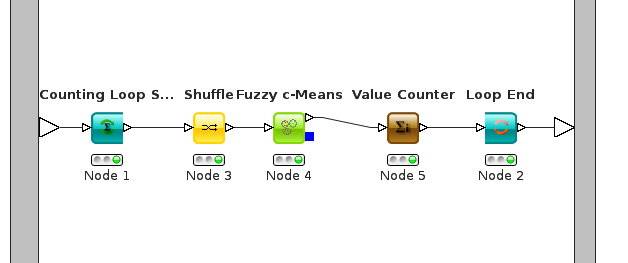
\includegraphics[width=13cm]{\PIXPATH/loop}
\end{figure}

Les deux figures suivantes montrent un clustering stable et instable sur
100 itérations. On voit que pour deux cluster recherchés, on trouvera
toujours trois cluster (clustering stable). En revanche, en recherchant
quatre cluster, le nombre de clusters trouvés varie grandement entre les
différentes itérations : le clustering est instable.

\begin{figure}[h]
\centering
\caption{Clustering stable et instable}
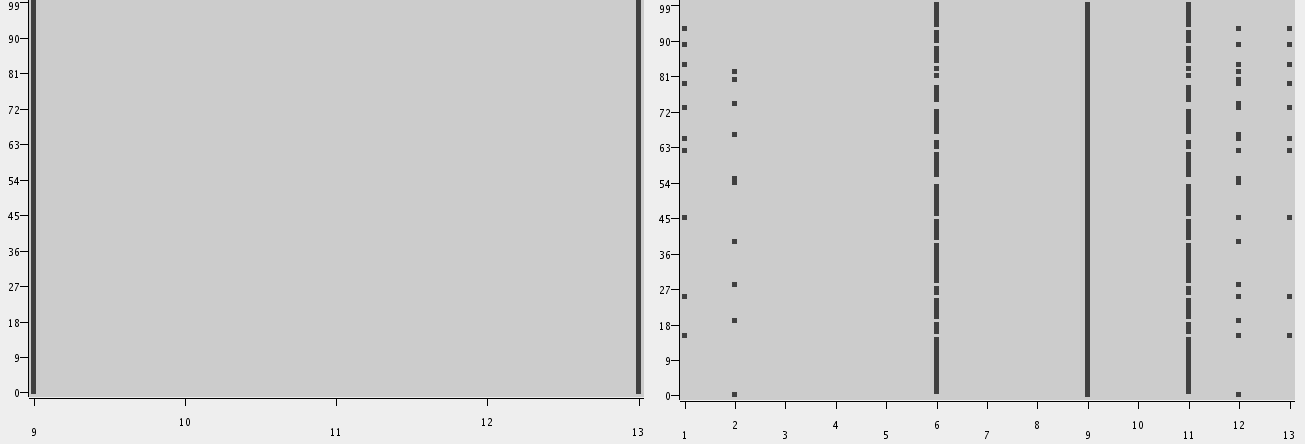
\includegraphics[width=13cm]{\PIXPATH/scatter_ok}
\end{figure}


\subsubsection{Clustering basé sur les secteurs d'activité}

On cherche à classer les pays selon la part des différents secteurs
(primaire, secondaire, tertiaire) au PIB. À cette fin, on retient les
attributs suivants :
\begin{itemize}
\item Agriculture, value added (\% of GDP)
\item Industry, value added (\% of GDP)
\item Services, etc., value add (\% of GDP)
\item GDP per capita (current US\$)
\end{itemize}

\vskip 6pt

L'emploi de l'attribut GDP per capita, au lieux du GDP, permet de disposer
d'un indice rapporté au nombre d'habitants du pays (autrement, les pays
"riches" mais petits ou faiblement peuplés et donc avec un faible GDP, ne
seraient pas correctement traités).

\paragraph{Conclusion}\hfill\\

Nous déterminons trois clusters. On présente la matrice des différents
nuages de points ci-après.

\begin{sidewaysfigure}[h]
\centering
\caption{Première approche de clustering}
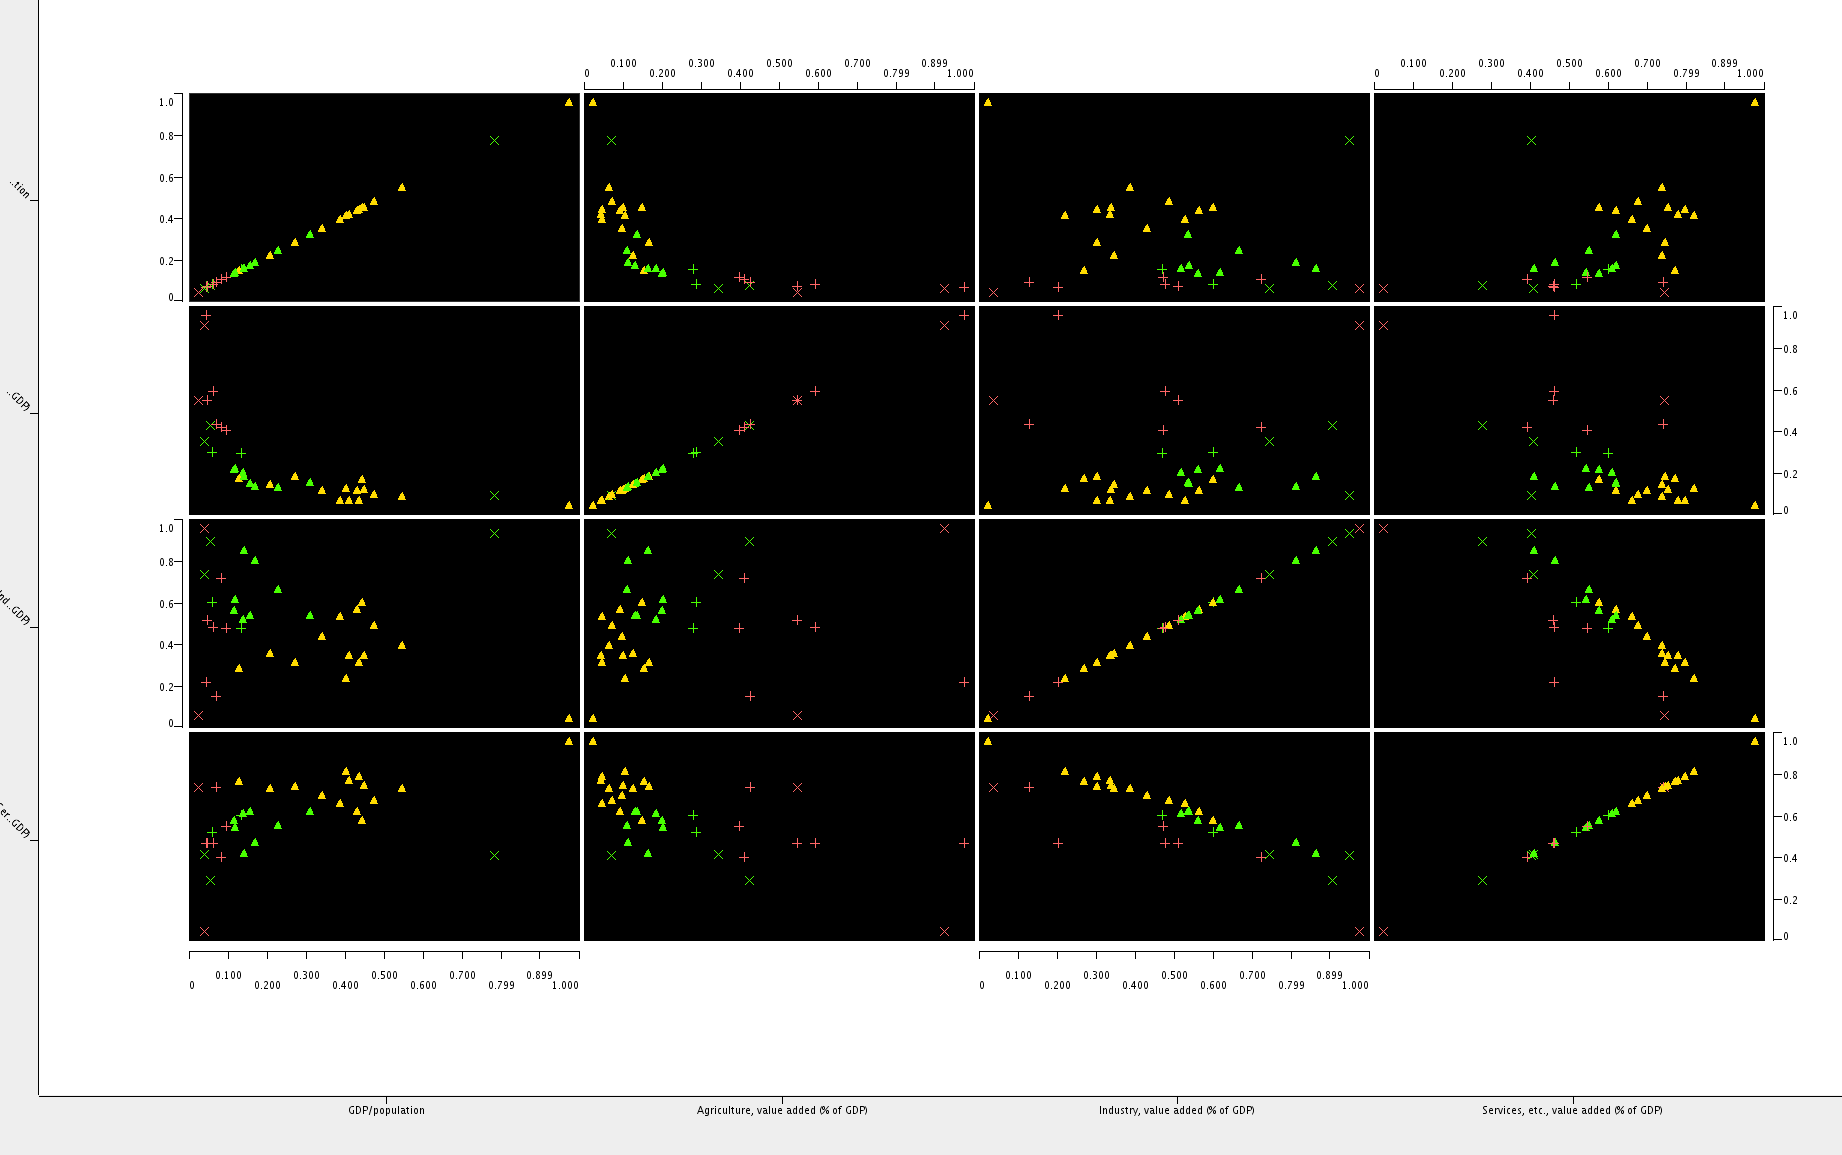
\includegraphics[width=22cm]{\PIXPATH/secteurs_matrix}
\end{sidewaysfigure}

Les clusters peuvent être caractérisés comme suit :
\begin{description}
\item[Cluster Jaune : ] Pays au meilleur niveau de vie et à forte activité de services (industrie moyenne et agriculture faible)
\item[Cluster Vert : ] Pays au niveau de vie intermédiaire, les mieux placés dans l'activité industrielle (services moyens et agriculture faible)
\item[Cluster Rouge :] Pays au niveau de vie le plus faible, à activité agricole principalement

\vskip 6pt

On peut voir que tous les pays membres de l'UE sont présents dans les deux
premiers clusters. Les pays candidats sont situés en majorité dans le cluster rouge
(Turquie, Albanie, Macédoine, Monténégro, Roumanie, Serbie, Turquie). Deux candidats
sont situés dans le cluster jaune (Bulgarie, Croatie).\\
Les pays non-candidats sont répartis entre le premier cluster (pays riches tels que la Norvège)
et le dernier (pays d'Europe de l'Est).\\
Enfin, il est également intéressant de constater que dans les deux premiers clusters,
les pays membres sont répartis en fonction de leur ancienneté dans l'UE (l'UE des 15
est dans le cluster jaune, et les pays ajoutés à l'UE des 27 constituent la majeur
partie du cluster vert).


\subsubsection{Clustering basé sur la santé publique}

On cherche à classer les pays selon la santé de leurs citoyens. Pour cela
on s'appuie sur les indicateurs suivants :

\begin{itemize}
\item Immunization, meastles (\% of children ages 12-23 months)
\item Life expectancy at birth, total (years)
\item Mortality rate, under-5 (per 1000)
\item Prevalence of HIV, total (\% of population ages 15-49)
\end{itemize}

\paragraph{Conclusion}\hfill\\

Là aussi, on détermine trois clusters :

\begin{sidewaysfigure}[h]
\centering
\caption{Deuxième approche de clustering}
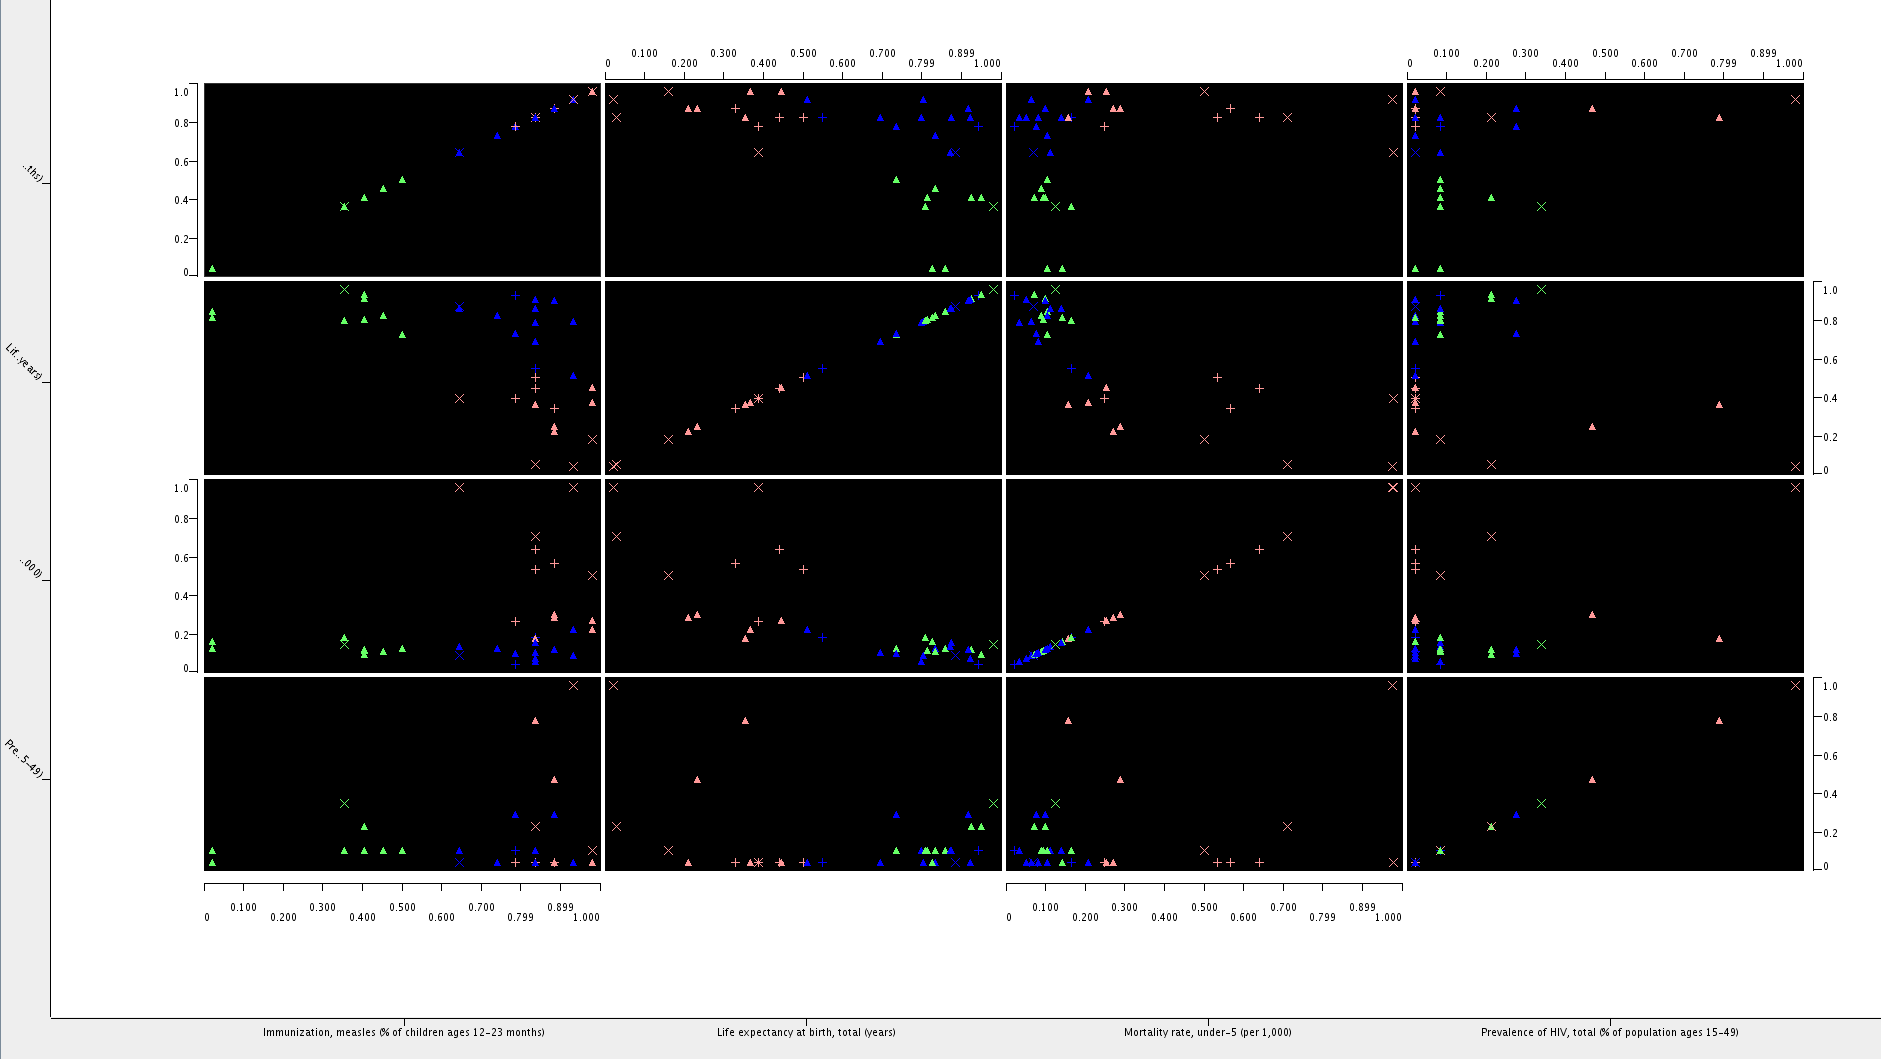
\includegraphics[width=22cm]{\PIXPATH/sante_matrix}
\end{sidewaysfigure}

\begin{description}
\item[Cluster Bleu : ] Pays en bonne santé (meilleur accès aux vaccins, meilleure espérance de vie, plus faible taux de mortalité infantile, faible taux de SIDA)
\item[Cluster Vert : ] Pays similaires à ceux du cluster bleu, mais avec un moins bon accès aux vaccins
\item[Cluster Rouge : ] Pays en moins bonne santé (bon accès aux vaccins mais espèrance de vie la plus faible et mortalité infantile la plus forte, associé à un fort taux de SIDA)
\end{description}

\vskip 6pt

Cette fois-ci, on ne retrouve pas une marque d'appartenance ou non à l'UE dans
le clustering. En revanche, il est intéressant de constater que les cluster bleu
et vert regroupent tous les pays de l'Europe de l'Ouest tandis que le cluster rouge
est exclusivement composé de pays de l'Est (ex-bloc soviétique), à l'exception de
la Pologne et de la Croatie (situés dans le cluster vert).


\subsubsection{Clustering basé sur la consommation et la production de
Hautes Technologies}

On cherche à classer les pays selon l'usage des HT par les citoyens :
consommation et production.

\begin{itemize}
\item High-technology exports (\% of manufactured exports)
\item Internet users (per 100 people)
\item Mobile cellular subscription (per 100 people)
\end{itemize}

\paragraph{Conclusion}\hfill\\

Ici aussi, on détermine trois clusters.

\begin{sidewaysfigure}[h]
\centering
\caption{Troisième approche de clustering}
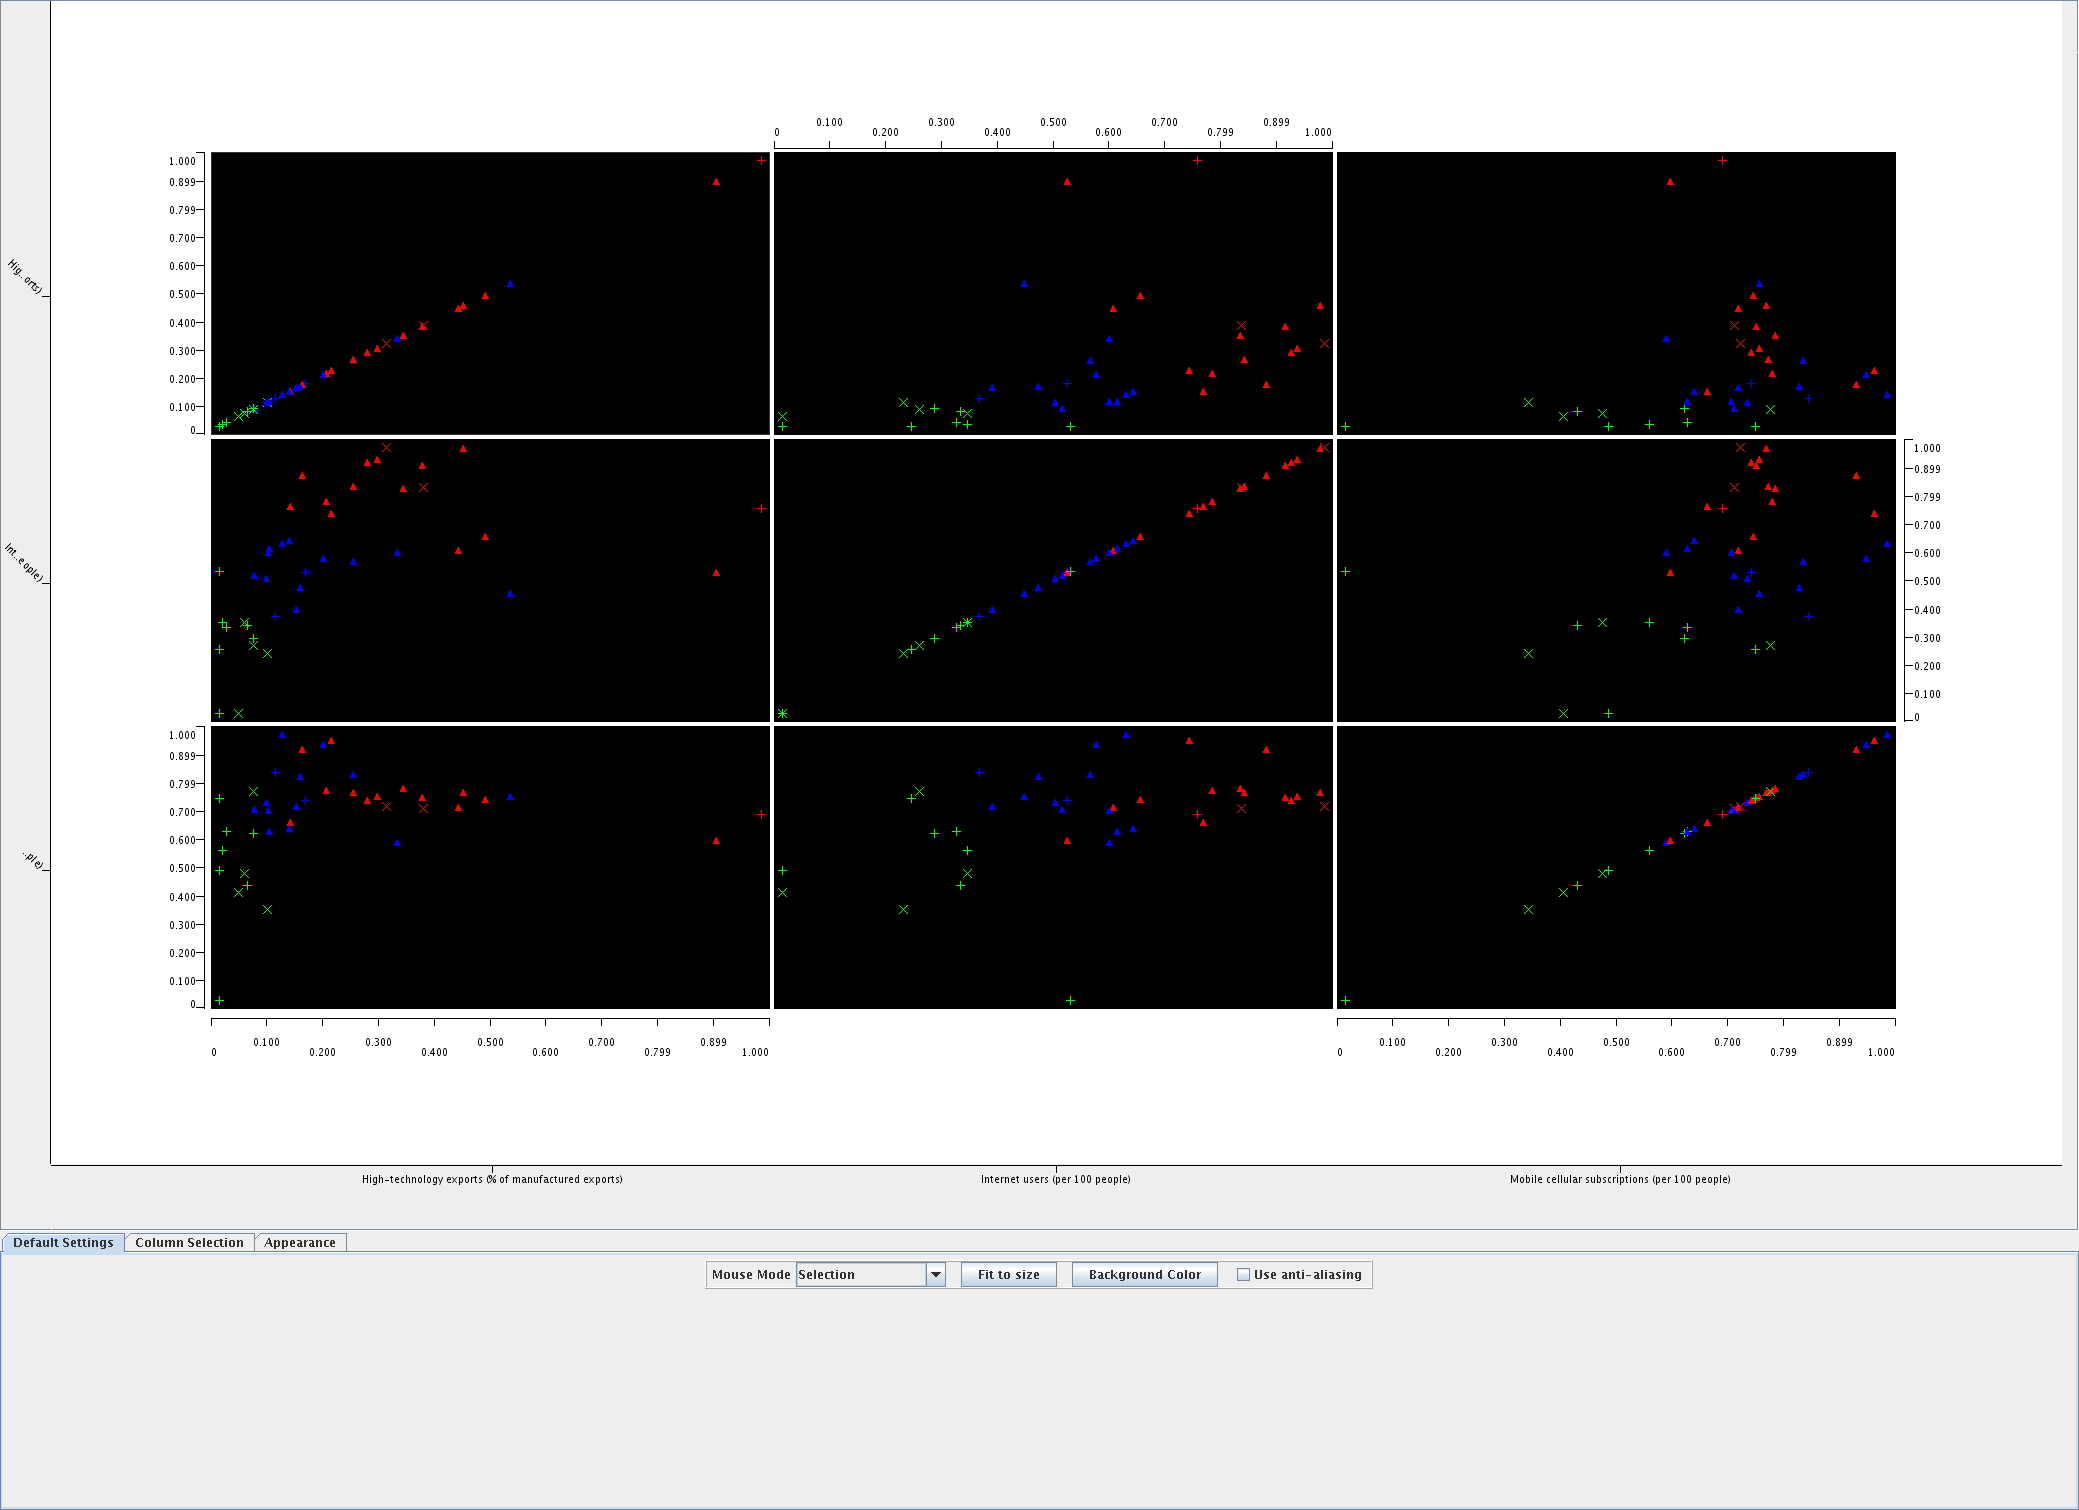
\includegraphics[height=22cm]{\PIXPATH/techno_matrix}
\end{sidewaysfigure}

\begin{description}
\item
\end{description}

\subsection{Conclusion sur les essais de clustering}
